
\paragraph{Architecture of the convolutional VAE}
Our implementation of the convolutional VAE  (CVAE) is similar in architecture to the original VAE\@. The primary difference between the two models is that the two linear layers in the encoder and decoder part of the original VAE have been replaced by respectively two convolutional layers and two transposed convolutional layers in the convolutional VAE\@. The two convolutional layers in the encoder part of the CVAE both use kernels of size $3\times 3$, $1\times 1$ padding and a stride of $2\times2$. The first convolutional layer has $1$ input channel and $16$ output channels, while the second convolutional layer has $16$ input channels and $32$ output channels. \iffalse As such, each convolutional layer decreases the spatial dimensions of their input by a factor of $2$, and the second convolutional layer additionally increases the feature dimension of its input by a factor $2$ to offset the loss in spatial dimensions. \fi The transposed convolutional layers in the decoder part of the CVAE complement the aforementioned convolutional layers. Both transposed convolutional layers use kernels of size $3\times3$, $1\times 1$ padding, $1\times 1$ output padding and a stride of $2\times 2$. The first transposed convolutional layer has $32$ input channels and $16$ output channels, while the second transposed convolutional layers has $16$ input channels and $1$ output channel. \iffalse As such, each transposed convolutional layers "undoes" the spatial reduction produced by a corresponding prior convolutional layer by upsampling the spatial dimensions of its input with a factor of $2$. \fi Conceptually, the encoder part of the CVAE condenses its input images $\mathbf{x}$ of size $D = H \times W$ into a compact but feature rich representation $\mathbf{z}$ of size $C = 2$, while the corresponding decoder "unfolds" this compact representation in reverse order, ultimately producing output images $\mathbf{y}$ of the same size as $\mathbf{x}$. 
\paragraph{Parameter estimation}
In order to optimize the CVAE model we estimate the parameters $\bm{\phi}$ and $\bm{\theta}$ that maximize the ELBO, which is a lower bound on the log likelihood of the data $\mathbf{x}$ and is defined as $\mathcal{L}(\bm{\theta}, \bm{\phi}, \mathbf{x}) = \E_{q_{\bm{\phi}}(\mathbf{z}|\mathbf{x})}{\lrs{\ln{p_{\bm{\theta}}(\mathbf{x} |\mathbf{z} )}}} - \KL (q_{\bm{\phi}}(\mathbf{z}|\mathbf{x}) \lVert p_{\bm{\theta}}(\mathbf{z}) )$. This is the same criterion used to optimize the original VAE\@. In particular, both models use the reparameterization trick to sample latent variables $\mathbf{z}$ from a factorized gaussian approximate posterior $q_{\bm{\phi}}(\mathbf{z}|\mathbf{x}) = \mathcal{N}(\mathbf{z}; \mathbf{u}, \text{diag}(\bm{\sigma}^2))$, so the Kullback-Leibler divergence, which acts as a regularization term in the ELBO, simplifies to $\frac{1}{2}\sum_{d=1}^{D}(\sigma_d^2 + \mu_d^2 - 1 - \ln(\sigma_d^2))$, assuming that the prior over $\mathbf{z}$ is also a diagonal gaussian $p_{\theta}(\mathbf{z}) = \mathcal{N}(\mathbf{z};\mathbf{0}, \mathbf{I})$. Here $\ln{\bm{\sigma}^2}$ and $\bm{\mu}$ are the outputs of the encoder when applied to $\mathbf{x}$. In order to compute the first term in the ELBO, which is the expected likelihood of $\mathbf{x}$ given $\mathbf{z}$, we utilize the output $\mathbf{y}$ of the decoder. We fed $\mathbf{y}$ through a sigmoid activation layer, which produces the mean parameters $\mathbf{p}$ of a factorized multivariate Bernoulli distribution $\prod_j^{D} \text{Bernoulli}(x_j; p_j)$ acting as the likelihood $p_{\bm{\theta}}(\mathbf{x} |\mathbf{z} )$ of the input $\mathbf{x}$ given latent variable $\mathbf{z}$. \iffalse As such, one may regard both VAE models as making the simplifying assumption that the MNIST data is binary, which is not technically the case. The simplifying assumption is most likely warranted given that the vast majority of pixels in the MNIST dataset are in fact either $0$ or $1$. Given this simplification , \fi We then approximate  the expected log likelihood by computing the negative of the binary cross entropy of $\mathbf{p}$ and $\mathbf{x}$, where $\mathbf{x}$ is treated as a set of probability values. Given the simplified ELBO, we optimize the parameters of both models using a variant of gradient descent, namely the Adam algorithm with a learning rate of $0.001$ and a batch size of $128$. In order to ensure convergence we run the Adam algorithm for a total of $25$ epochs for each model. We train both models on the complete MNIST training set.

\paragraph{Performance of VAE models}
We compare the performance of the two VAE models on the MNIST test set using two quantitative measures and three qualitative experiments. The two quantitative measures are the sample-wise mean ELBO on the MNIST test set and the MSE loss between samples from the MNIST test set and corresponding reconstructions produced by the VAE models. The three qualitative experiments are
\begin{enumerate}
    \item Clustering MNIST test data in latent space by mapping each observation $\mathbf{x}_i$ to corresponding mean parameters $\bm{\mu}_i$ using the encoder and subsequently plotting these $\bm{\mu}_i$ with colors based on the actual labels $t_i$ associated with each $\mathbf{x}_i$.
    \item Exploring the latent space by sampling latent variables $\mathbf{z}$ deterministically from a regular grid, then using the decoder to map these $\mathbf{z}$ to corresponding mean parameters $\mathbf{p}$,  and finally visualizing these $\mathbf{p}$ as images.
    \item Reconstructing selected observations $\mathbf{x}_i$ from the MNIST test set by mapping these to posterior distributions $q_{\bm{\phi}}(\mathbf{z}_i|\mathbf{x}_i)$, then randomly sampling $\mathbf{z}_i$ from these posterior distributions, and finally using the decoder to map these $\mathbf{z}_i$ to corresponding mean parameters $\mathbf{p}_i$, which are finally interpreted as reconstruction of the inputs $\mathbf{x}_i$.
\end{enumerate}
A comparison of the sample-wise ELBO and MSE loss for the two VAE models is shown in \cref{table:metrics}. As can be seen, both models seem to have a sample-wise mean ELBO that is on the same scale as well as an MSE loss that is on the same scale. However, it is also apparent that both the sample-wise mean ELBO and the MSE loss is slighter better for the original VAE than for the CVAE\@. This indicates the VAE has learned a slightly better approximation of the density implicitly defined by the MNIST test set as well as being slightly better at reconstructing images from the MNIST test set. The clustering of the MNIST test data shown in \cref{fig:vae:clustering} and \cref{fig:cvae:clustering} indicate a similar relationship between the performance of the two models. In particular, we see that both models seem to have learned a representation in latent space that is capable of separating most samples from the MNIST test set based on class labels. That being said, it also clear that the CVAE struggles more than the VAE with separating some samples based on class labels, in particular those representing digits 4, 7, and 9. 

The exploration of latent space shown in \cref{fig:vae:interpolation} and \cref{fig:cvae:interpolation} corroborate the idea that the VAE is better at separating classes. Note in particular how the mean parameter images produced by the VAE seem to be slightly more well-defined (i.e.\ less blurry) than those produced by the CVAE\@. It is also worth noting that the exploration of latent space in the CVAE seem to produce a greater variety of digits than does the corresponding exploration of latent space in the VAE (it seems to mainly produce 6s, 0s, 2s, 1s and 9s). The reconstruction results shown in \cref{fig:vae:mean} and \cref{fig:cvae:mean} also indicate that the VAE is somewhat superior to the CVAE, in this case in terms of accurately reconstructing samples from the MNIST test set. This is most obvious when considering the reconstructions of digits 2 and 4, which the VAE has rendered reasonably clearly, contrary to the CVAE, which has rendered them somewhat blurry. In particular, it seems that the CVAE has trouble distinguishing 4 from 9. 

The reason why the CVAE slightly underperforms compared to the VAE is not entirely clear to us. In fact, one might expect the CVAE would perform better than the VAE, given that convolutional layers in general are better than linear layers at capturing complex spatial information in image data. One reason why the CVAE underperforms may be that the MNIST dataset is too simple and hence convolutional layers are not required to extract its most salient features. In particular, since MNIST digits are centered and of similar size, the convolutional layers might not be necessary. Its also possible that the CVAE is not deep enough to effectively learn a useful representation of the MNIST data, that the kernel size ($3\times3$) used by its layers is not large enough to capture spatial dependencies in the MNIST data or that a stride of $(2\times2)$ results in too significant a loss of information. 

\begin{figure}%[h]
	\begin{floatrow}
	\captionsetup{width=.49\linewidth}
	\ffigbox{%
	\begin{subfigure}[t]{0.50\textwidth}
		\centering
		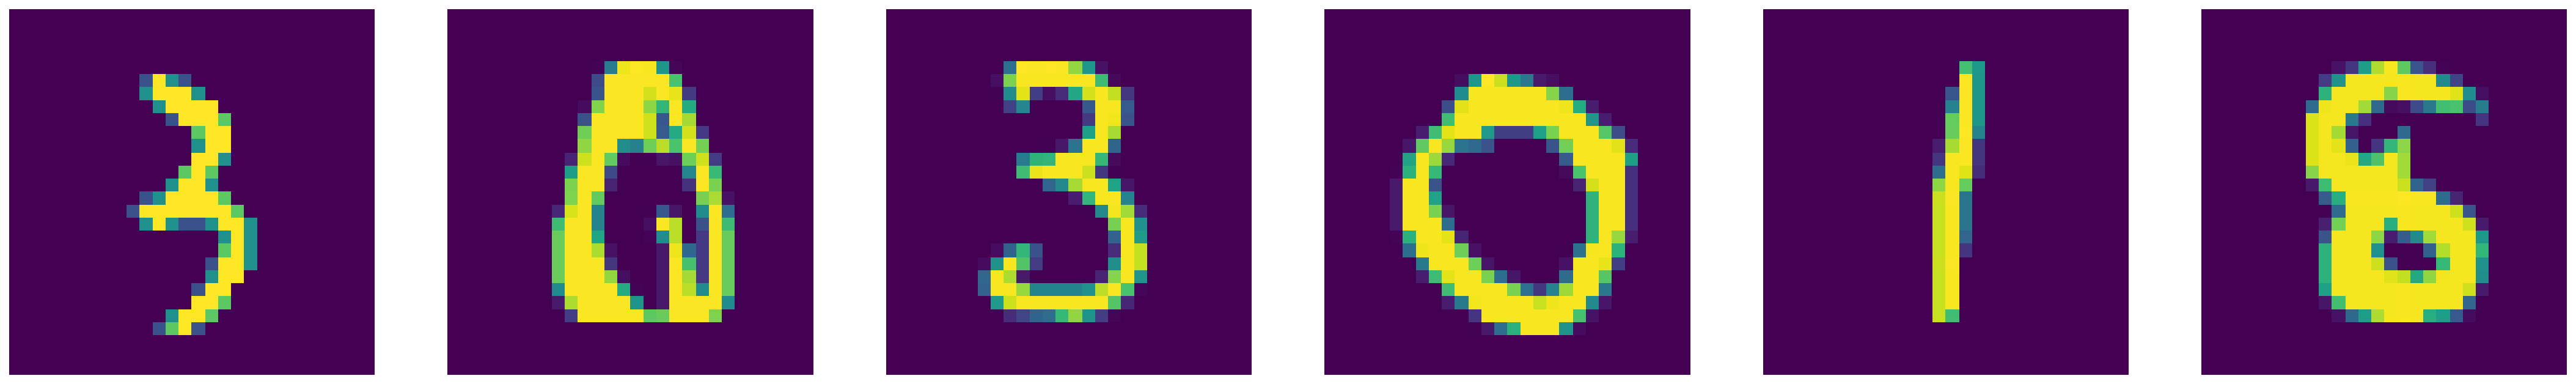
\includegraphics[width = 0.8\textwidth]{figures/ppca/real}
		\caption{Test set images}
		\label{fig:ppca:real}
	\end{subfigure}
	\begin{subfigure}[t]{0.5\textwidth}
		\centering
		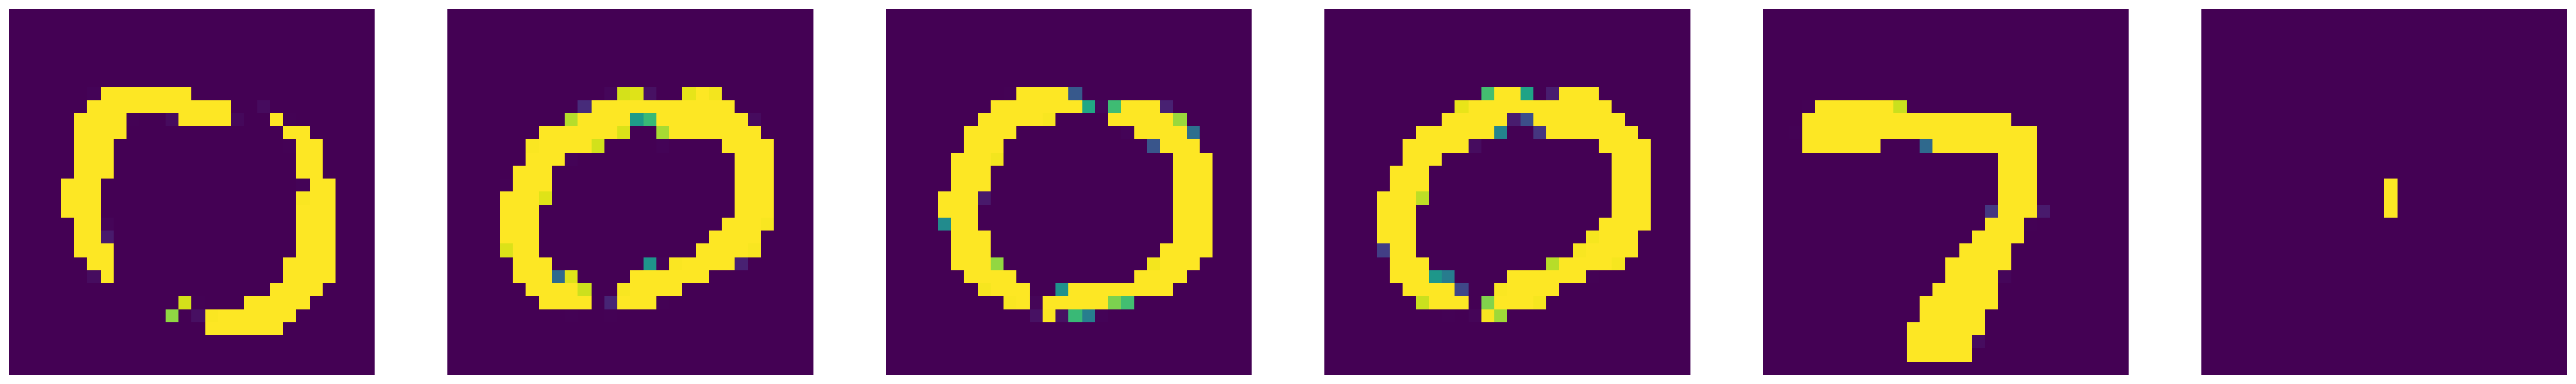
\includegraphics[width = 0.8\textwidth]{figures/vae/mean}
		\caption{VAE}
		\label{fig:vae:mean}
	\end{subfigure}
	\begin{subfigure}[t]{0.5\textwidth}
		\centering
		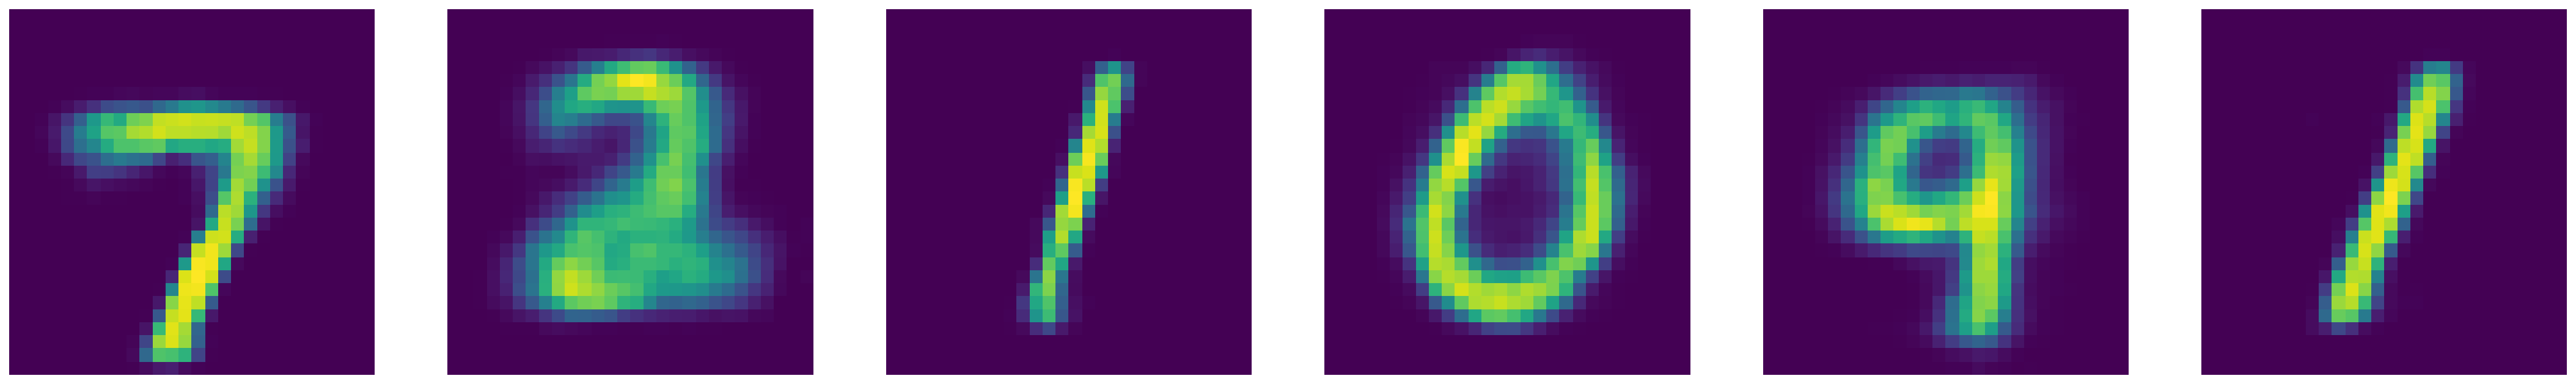
\includegraphics[width = 0.8\textwidth]{figures/cvae/mean}
		\caption{CVAE}
		\label{fig:cvae:mean}
	\end{subfigure}
	\begin{subfigure}[t]{0.5\textwidth}
		\centering
		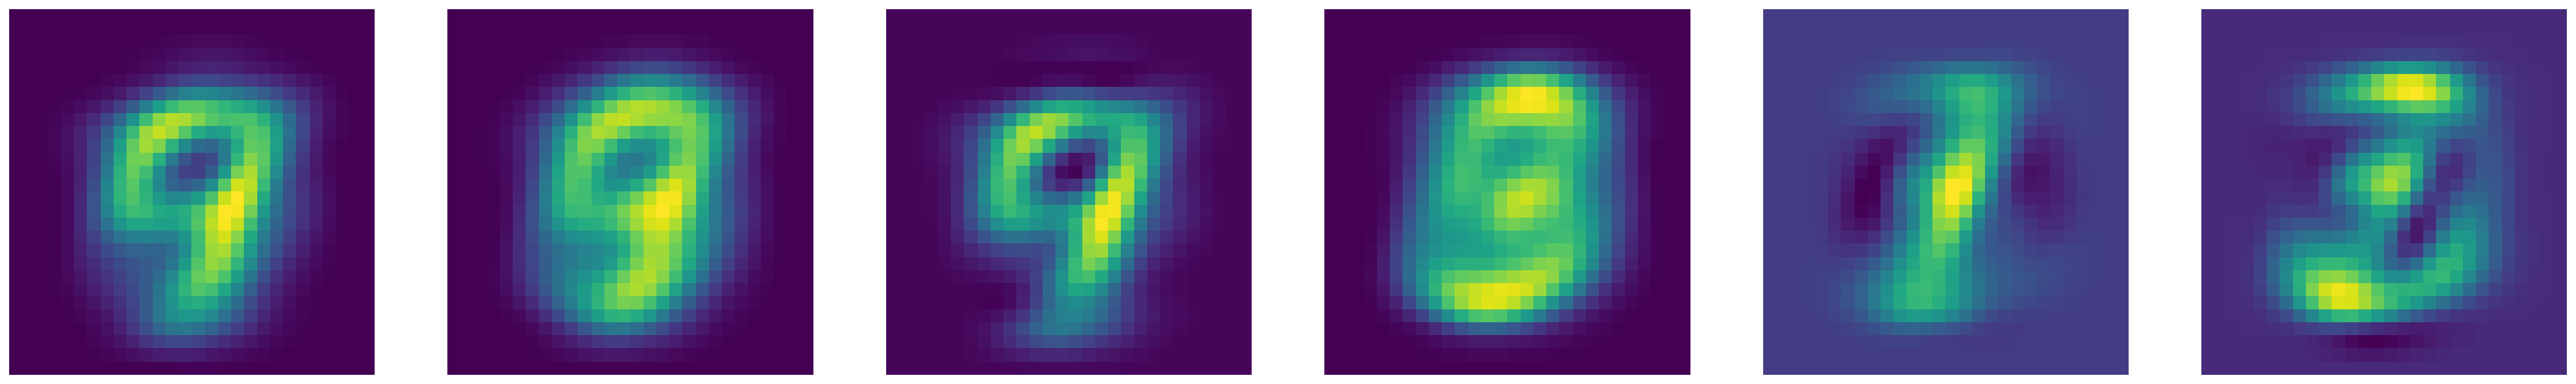
\includegraphics[width = 0.8\textwidth]{figures/ppca/mean}
		\caption{PPCA}
		\label{fig:ppca:mean}
	\end{subfigure}
	\begin{subfigure}[t]{0.5\textwidth}
		\centering
		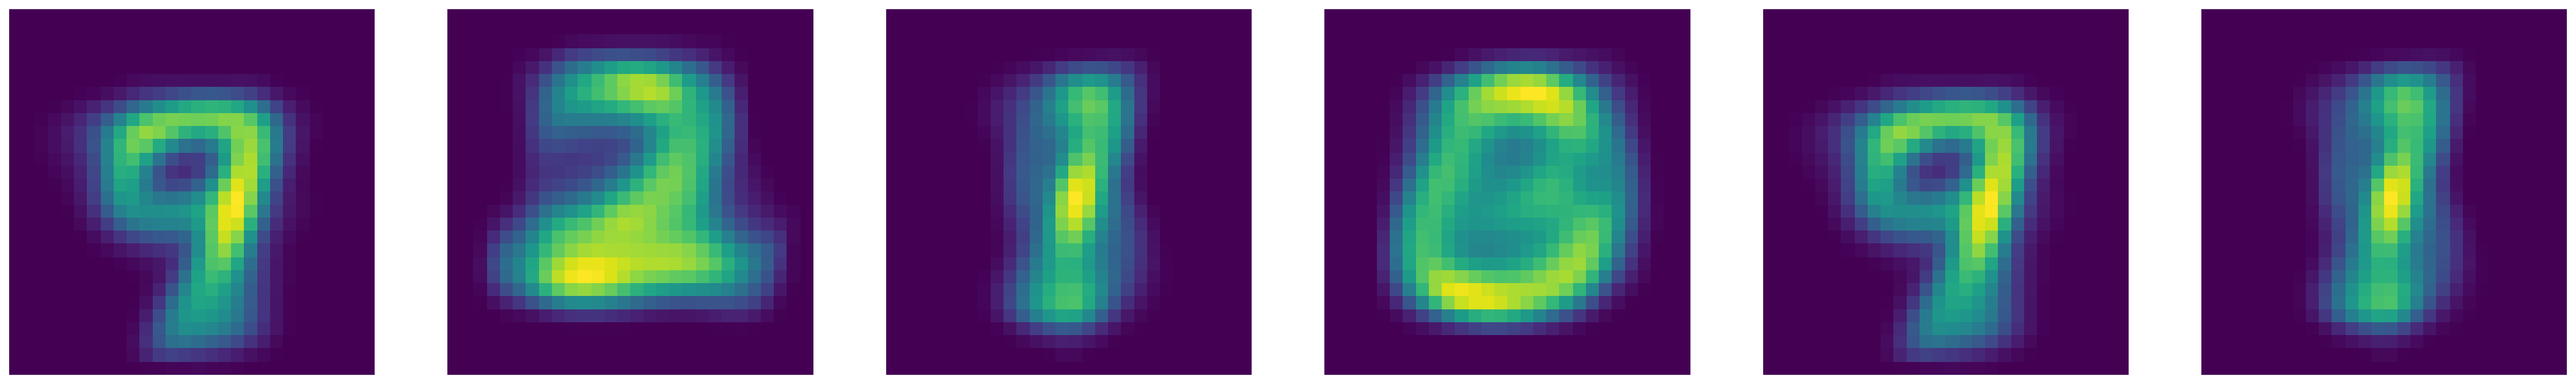
\includegraphics[width = 0.8\textwidth]{figures/gmm/mean}
		\caption{GMM}
		\label{fig:gmm:mean}
	\end{subfigure}
	
	}{%
	\caption{Comparison of MNIST test set images and corresponding mean parameters generated by density models.}
	}

	\capbtabbox{%
		\begin{tabular}{ccc}
		\toprule
		{} &  \textbf{Log-Likelihood/ELBO} &  \textbf{MSE} \\
		\midrule
		\textbf{VAE } &                 \num[round-mode=places,round-precision=4]{-1.428134e+02} &      \num[round-mode=places,round-precision=4]{0.037524} \\
		\textbf{CVAE} &                 \num[round-mode=places,round-precision=4]{-1.570527e+02} &      \num[round-mode=places,round-precision=4]{0.044375} \\
		\textbf{PPCA} &                 \num[round-mode=places,round-precision=4]{-4.329656e+03} &      \num[round-mode=places,round-precision=4]{0.055813} \\
		\textbf{GMM } &                 \num[round-mode=places,round-precision=4]{-1.066433e+07} &      \num[round-mode=places,round-precision=4]{0.058932} \\
		\bottomrule
		\end{tabular}
		
}{%
	\caption{Model performance metrics}
	\label{table:metrics}
}
	
	
\end{floatrow}
\end{figure}


\begin{figure}%[h]
	\begin{floatrow}
	\captionsetup{width=.49\linewidth}
	\ffigbox{%
	\begin{subfigure}[t]{0.45\textwidth}
		\begin{subfigure}[t]{0.49\textwidth}
			\centering
			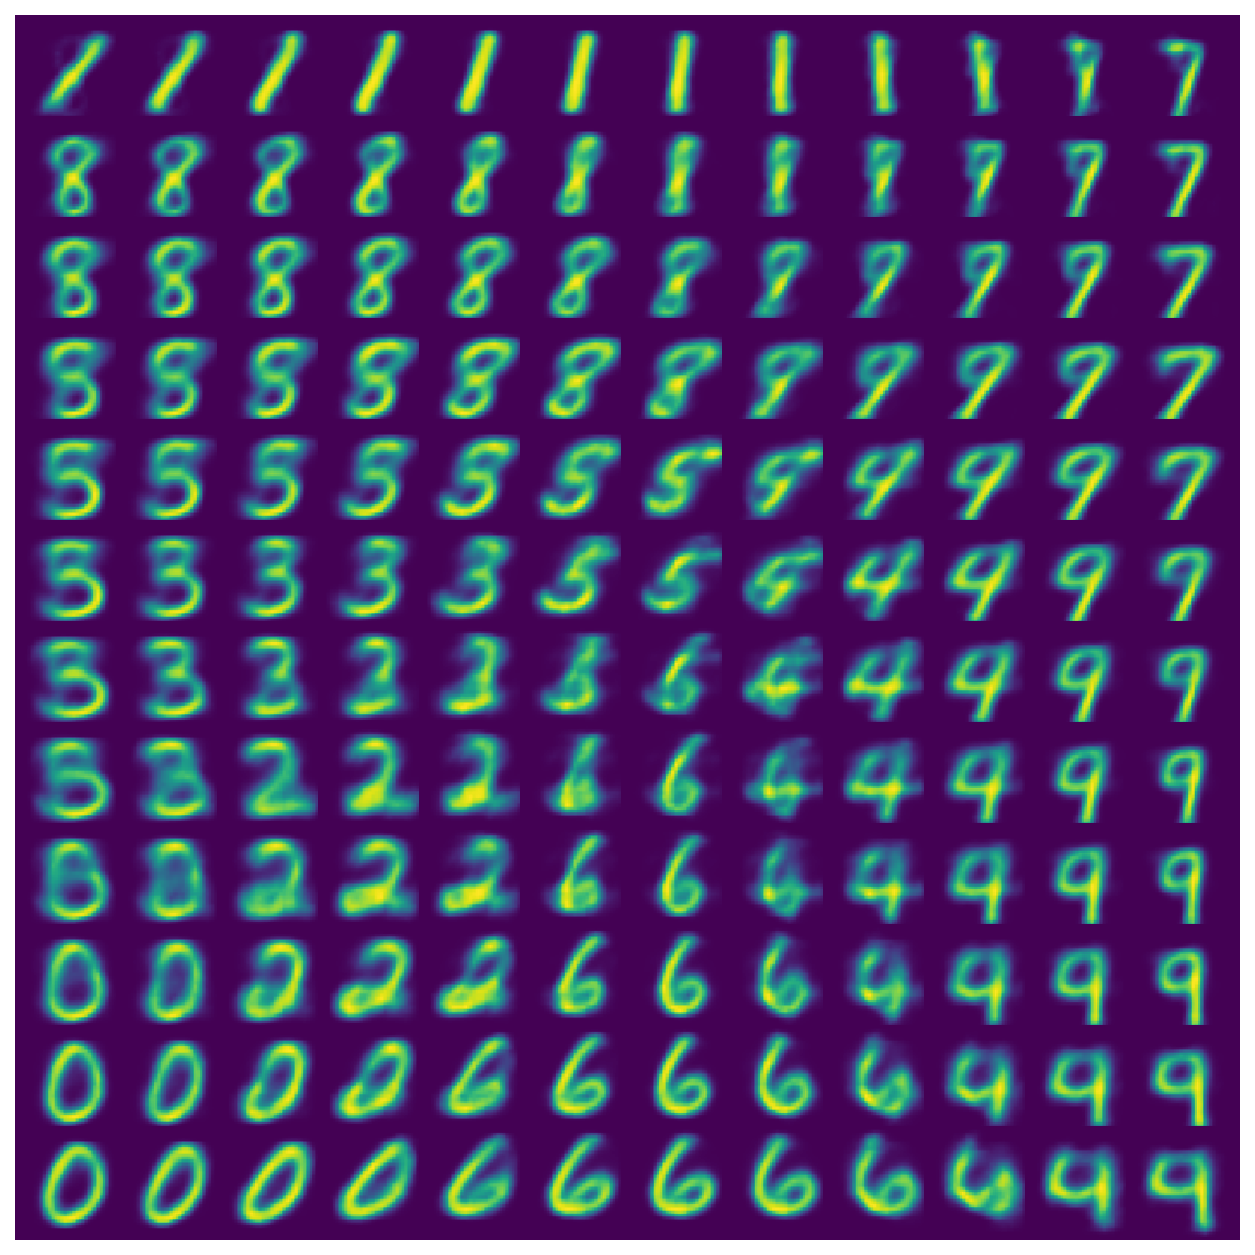
\includegraphics[width = 1\textwidth]{figures/vae/interpolation}
			\caption{VAE}
			\label{fig:vae:interpolation}
		\end{subfigure}
		\begin{subfigure}[t]{0.49\textwidth}
			\centering
			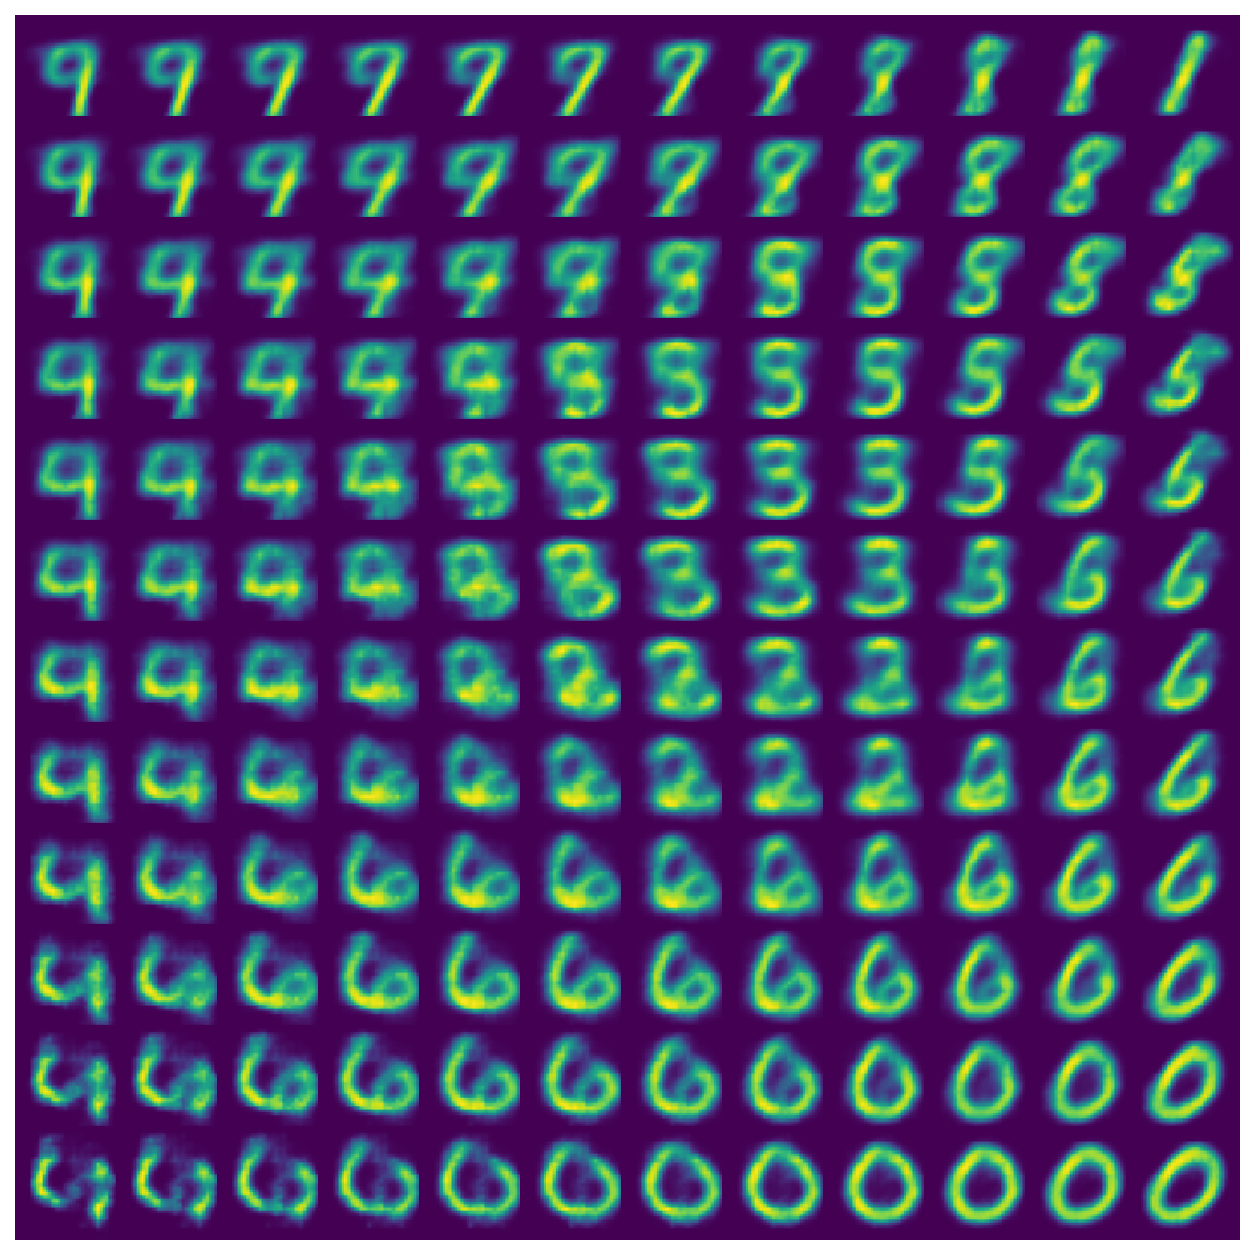
\includegraphics[width = 1\textwidth]{figures/cvae/interpolation}
			\caption{CVAE}
			\label{fig:cvae:interpolation}
		\end{subfigure}
		\begin{subfigure}[t]{0.49\textwidth}
			\centering
			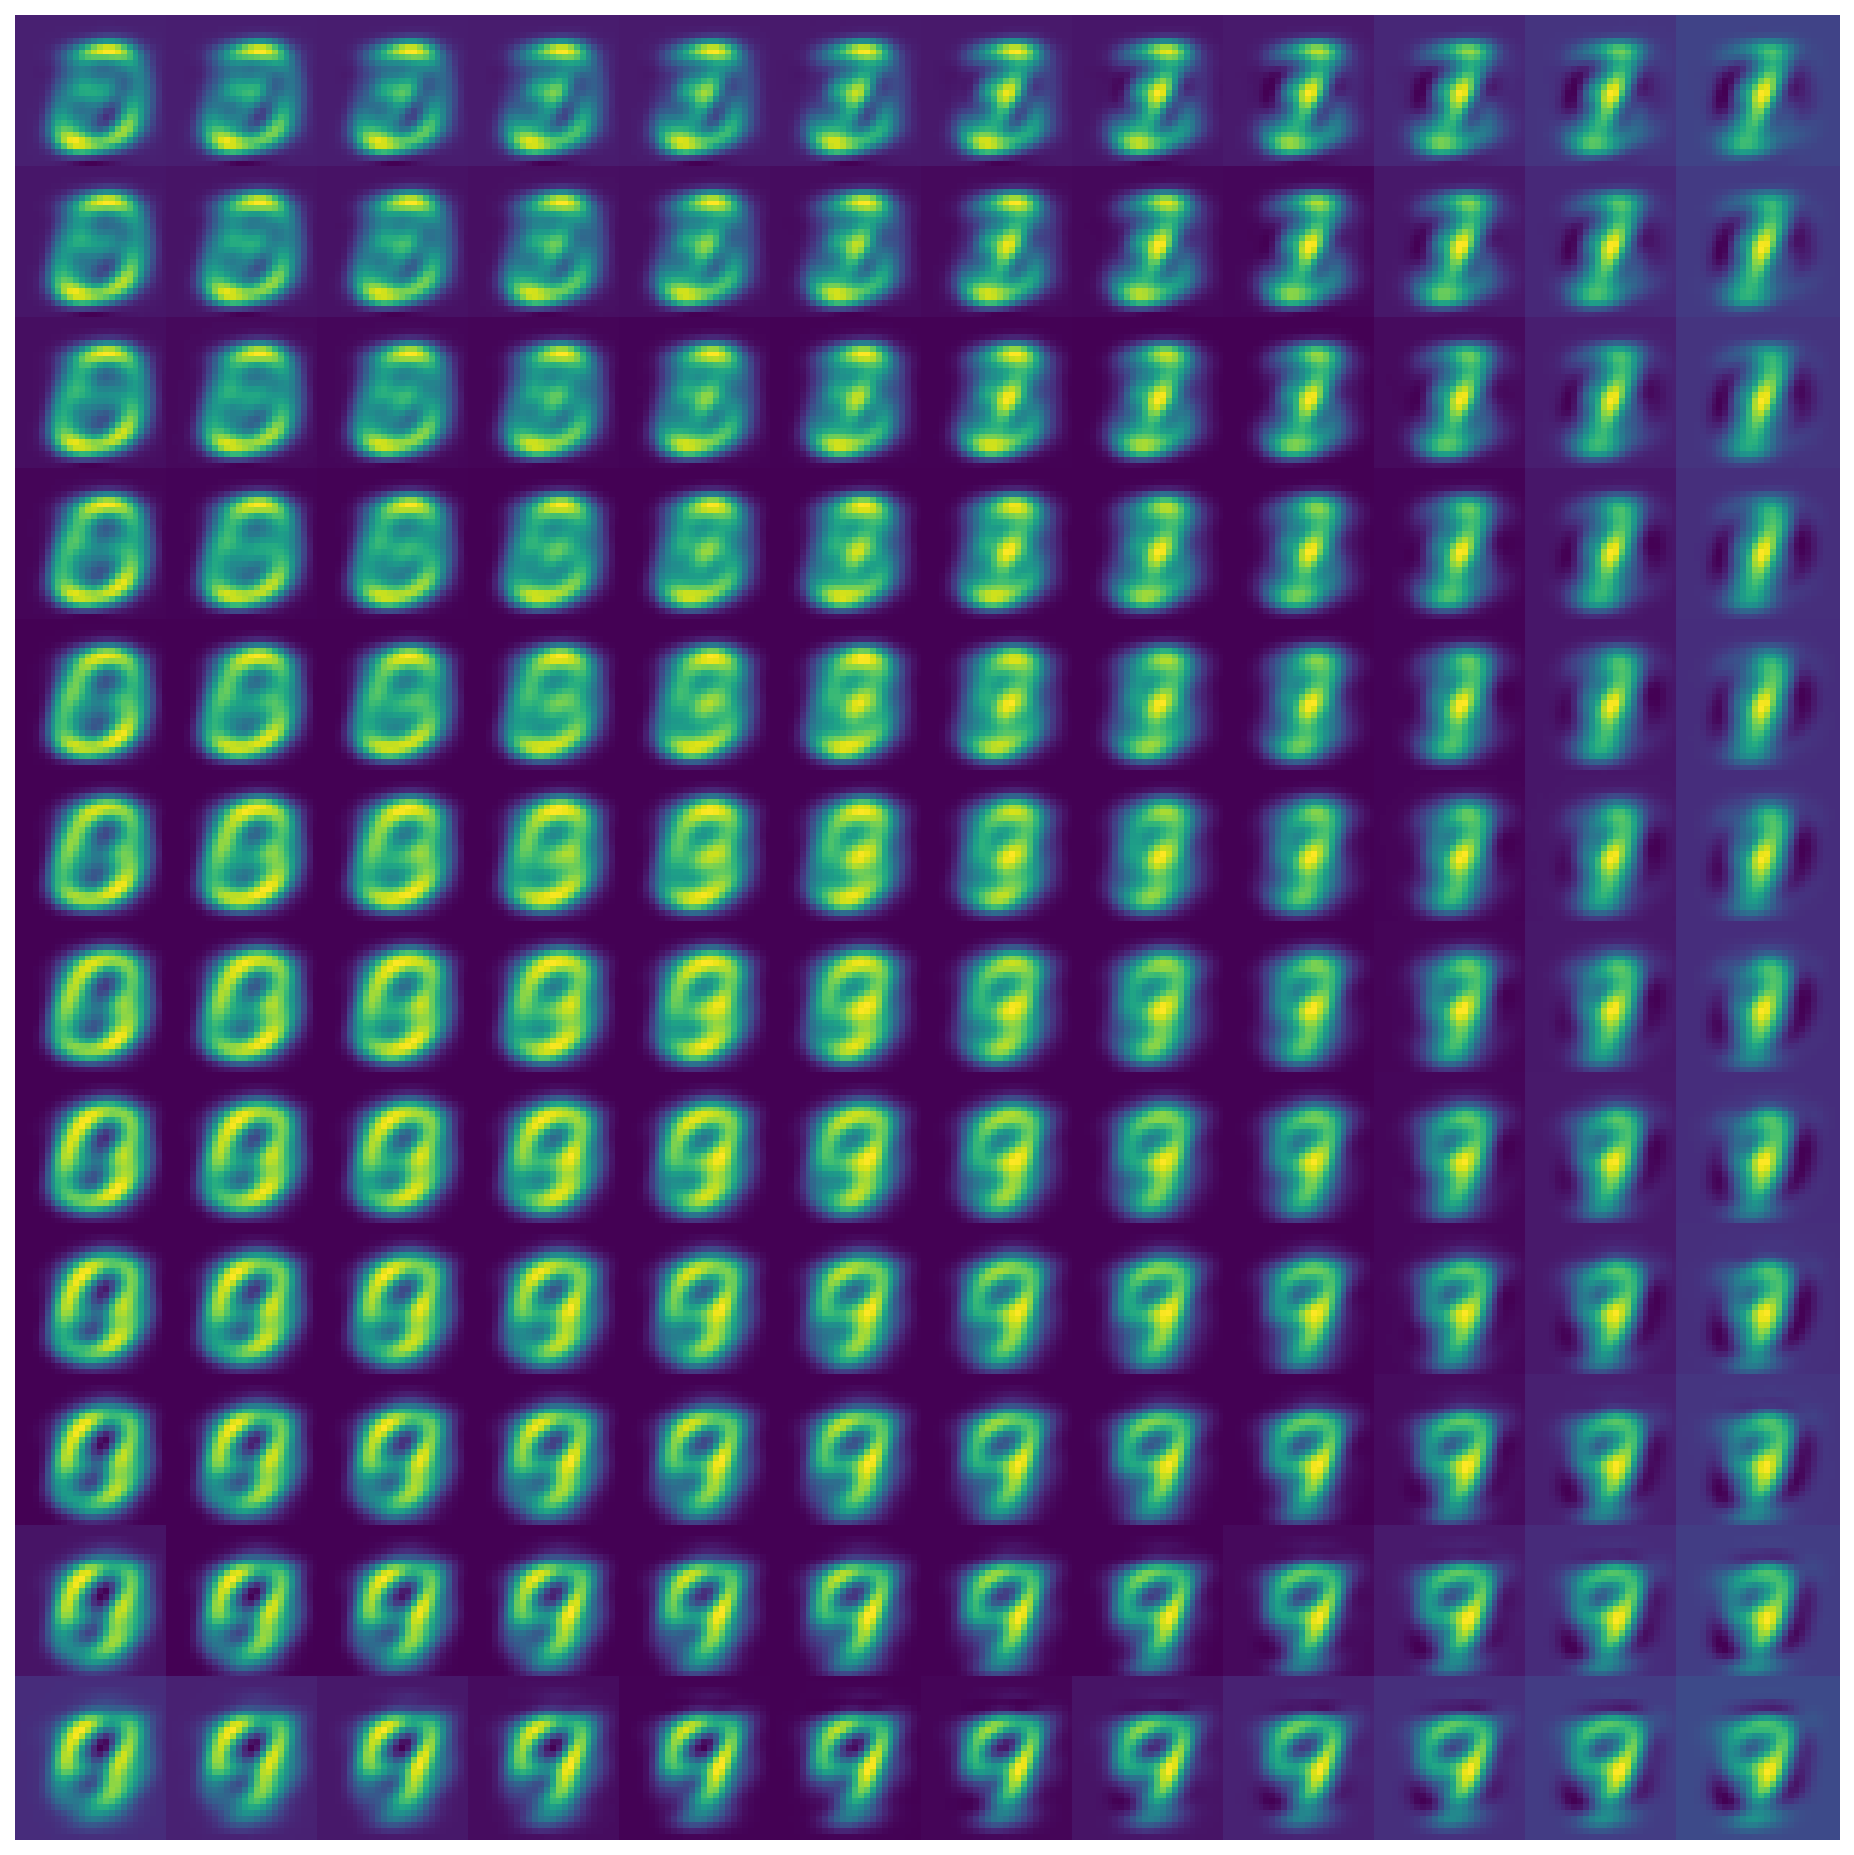
\includegraphics[width = 1\textwidth]{figures/ppca/interpolation}
			\caption{PPCA}
			\label{fig:ppca:interpolation}
		\end{subfigure}
		\begin{subfigure}[t]{0.49\textwidth}
			\centering
			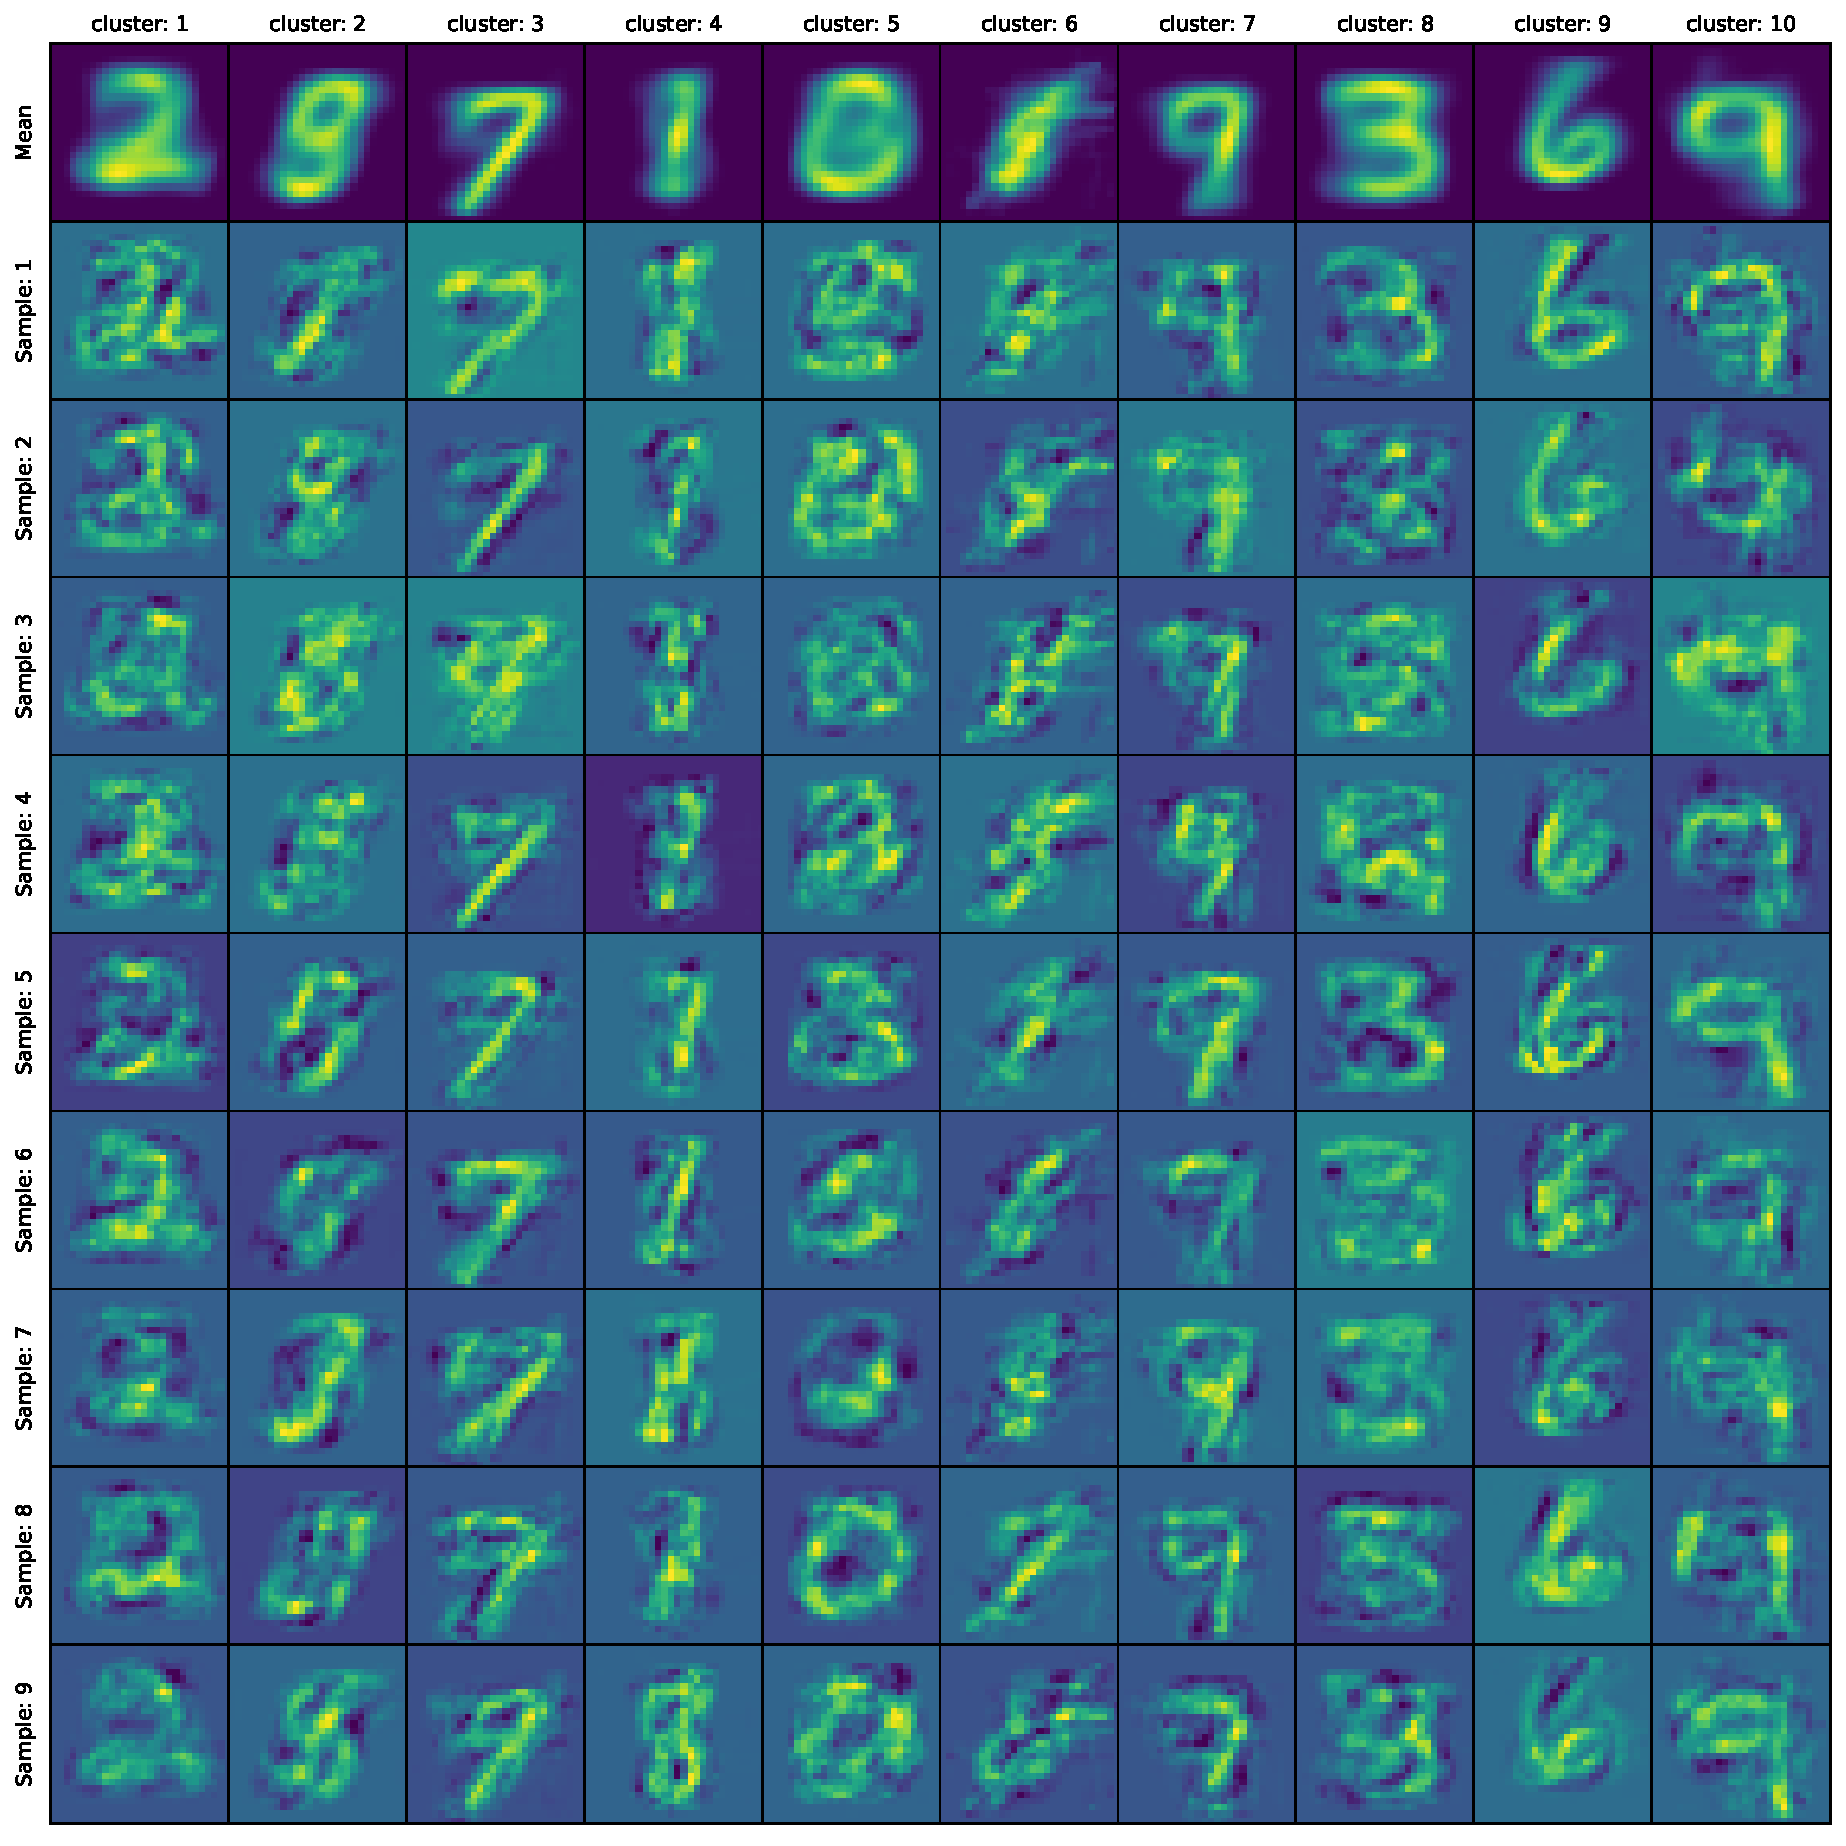
\includegraphics[width = 1\textwidth]{figures/gmm/interpolation}
			\caption{GMM}
			\label{fig:gmm:interpolation}
		\end{subfigure}	
	\end{subfigure}
	}{%
	\caption{Interpolating images from latent space variables using trained density models.}
	}
	\ffigbox{%
\begin{subfigure}[t]{0.45\textwidth}
		\begin{subfigure}[t]{0.49\textwidth}
			\centering
			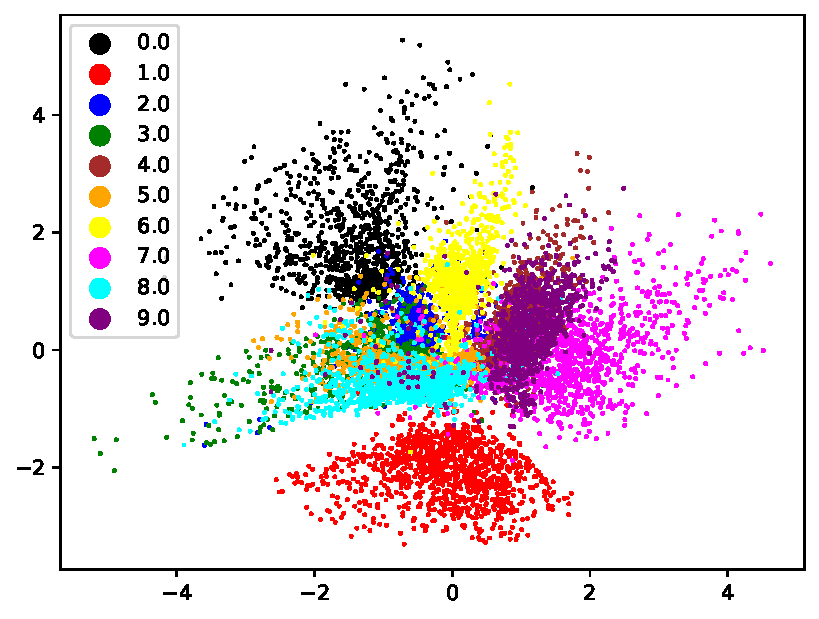
\includegraphics[width = 1\textwidth]{figures/vae/clustering}
			\caption{VAE}
			\label{fig:vae:clustering}
		\end{subfigure}
		\begin{subfigure}[t]{0.49\textwidth}
			\centering
			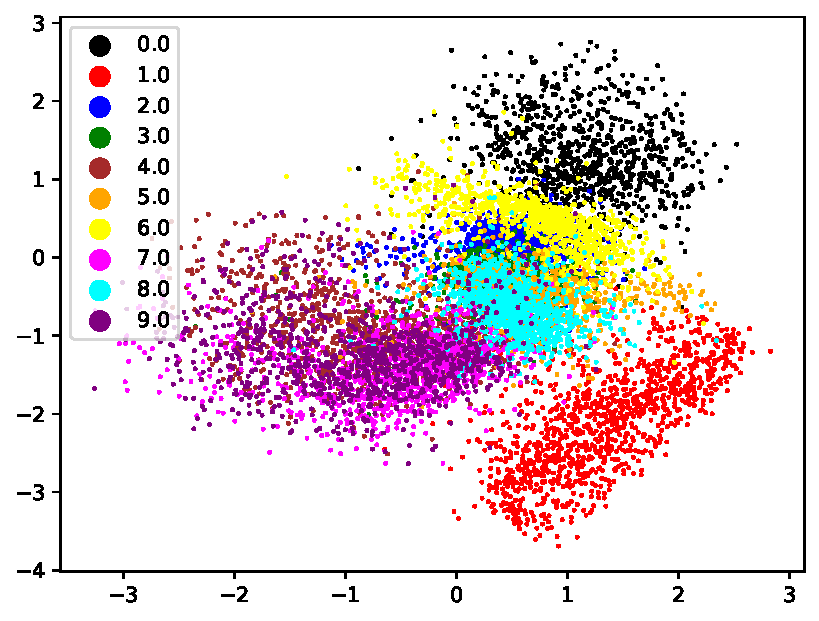
\includegraphics[width = 1\textwidth]{figures/cvae/clustering}
			\caption{CVAE}
			\label{fig:cvae:clustering}
		\end{subfigure}
		\begin{subfigure}[t]{0.49\textwidth}
			\centering
			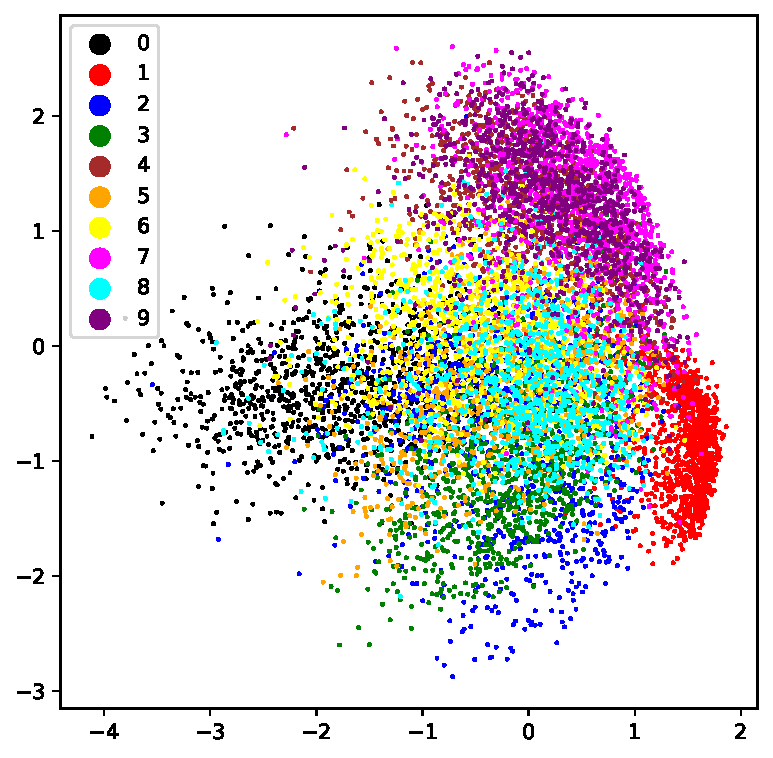
\includegraphics[width = 1\textwidth]{figures/ppca/clustering}
			\caption{PPCA}
			\label{fig:ppca:clustering}
		\end{subfigure}
		\begin{subfigure}[t]{0.49\textwidth}
			\centering
			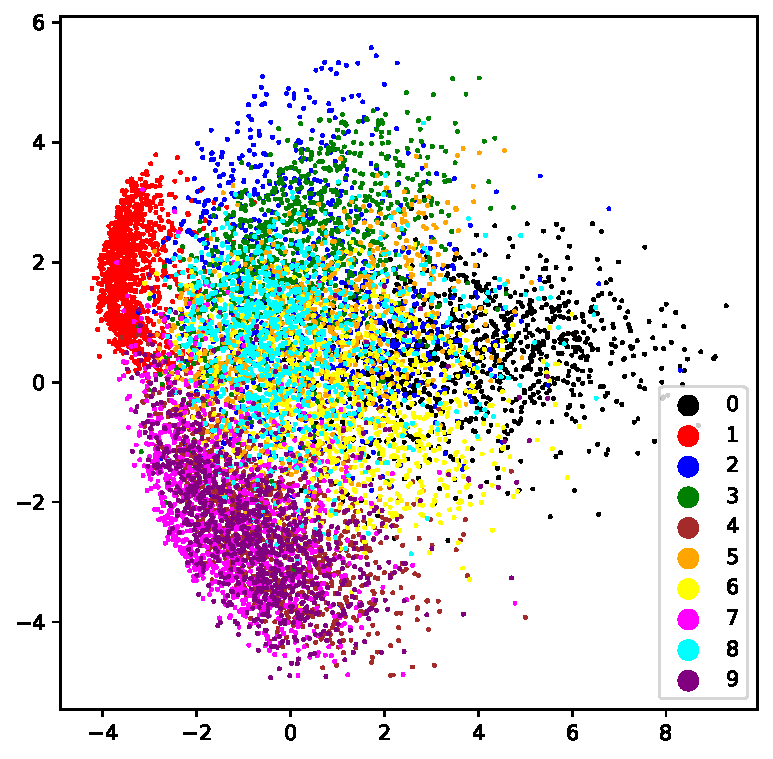
\includegraphics[width = 1\textwidth]{figures/gmm/clustering}
			\caption{GMM}
			\label{fig:gmm:clustering}
		\end{subfigure}
	\end{subfigure}
	}{%
	\caption{Clustering on MNIST test data (projection to latent space) using trained density models.}
	}
\end{floatrow}
\end{figure}